\documentclass[twoside]{article}
\setlength{\oddsidemargin}{0.25 in}
\setlength{\evensidemargin}{-0.25 in}
\setlength{\topmargin}{-0.6 in}
\setlength{\textwidth}{6.5 in}
\setlength{\textheight}{8.5 in}
\setlength{\headsep}{0.75 in}
\setlength{\parindent}{0 in}
\setlength{\parskip}{0.1 in}

\usepackage{graphicx}
\usepackage{url}

%
% The following commands sets up the lecnum (lecture number)
% counter and make various numbering schemes work relative
% to the lecture number.
%
\newcounter{lecnum}
\renewcommand{\thepage}{\thelecnum-\arabic{page}}
\renewcommand{\thesection}{\thelecnum.\arabic{section}}
\renewcommand{\theequation}{\thelecnum.\arabic{equation}}
\renewcommand{\thefigure}{\thelecnum.\arabic{figure}}
\renewcommand{\thetable}{\thelecnum.\arabic{table}}
\newcommand{\dnl}{\mbox{}\par}

%
% The following macro is used to generate the header.
%
\newcommand{\lecture}[4]{
  \pagestyle{myheadings}
  \thispagestyle{plain}
  \newpage
  \setcounter{lecnum}{#1}
  \setcounter{page}{1}
  \noindent
  \begin{center}
  \framebox{
     \vbox{\vspace{2mm}
   \hbox to 6.28in { {\bf COMPSCI~590S~~~Systems for Data Sciencea
                       \hfill Fall 2016} }
      \vspace{4mm}
      \hbox to 6.28in { {\Large \hfill Lecture #1: #2  \hfill} }
      \vspace{2mm}
      \hbox to 6.28in { {\it Lecturer: #3 \hfill Scribe(s): #4} }
     \vspace{2mm}}
  }
  \end{center}
  \markboth{Lecture {#1}: #2}{Lecture {#1}: #2}
  \vspace*{4mm}
}

%
% Convention for citations is authors' initials followed by the year.
% For example, to cite a paper by Leighton and Maggs you would type
% \cite{LM89}, and to cite a paper by Strassen you would type \cite{S69}.
% (To avoid bibliography problems, for now we redefine the \cite command.)
%
\renewcommand{\cite}[1]{[#1]}

% \input{epsf}

%Use this command for a figure; it puts a figure in wherever you want it.
%usage: \fig{NUMBER}{FIGURE-SIZE}{CAPTION}{FILENAME}
\newcommand{\fig}[4]{
           \vspace{0.2 in}
           \setlength{\epsfxsize}{#2}
           \centerline{\epsfbox{#4}}
           \begin{center}
           Figure \thelecnum.#1:~#3
           \end{center}
   }

% Use these for theorems, lemmas, proofs, etc.
\newtheorem{theorem}{Theorem}[lecnum]
\newtheorem{lemma}[theorem]{Lemma}
\newtheorem{proposition}[theorem]{Proposition}
\newtheorem{claim}[theorem]{Claim}
\newtheorem{corollary}[theorem]{Corollary}
\newtheorem{definition}[theorem]{Definition}
\newenvironment{proof}{{\bf Proof:}}{\hfill\rule{2mm}{2mm}}

% Some useful equation alignment commands, borrowed from TeX
\makeatletter
\def\eqalign#1{\,\vcenter{\openup\jot\m@th
 \ialign{\strut\hfil$\displaystyle{##}$&$\displaystyle{{}##}$\hfil
     \crcr#1\crcr}}\,}
\def\eqalignno#1{\displ@y \tabskip\@centering
 \halign to\displaywidth{\hfil$\displaystyle{##}$\tabskip\z@skip
   &$\displaystyle{{}##}$\hfil\tabskip\@centering
   &\llap{$##$}\tabskip\z@skip\crcr
   #1\crcr}}
\def\leqalignno#1{\displ@y \tabskip\@centering
 \halign to\displaywidth{\hfil$\displaystyle{##}$\tabskip\z@skip
   &$\displaystyle{{}##}$\hfil\tabskip\@centering
   &\kern-\displaywidth\rlap{$##$}\tabskip\displaywidth\crcr
   #1\crcr}}
\makeatother

% **** IF YOU WANT TO DEFINE ADDITIONAL MACROS FOR YOURSELF, PUT THEM HERE:



% Some general latex examples and examples making use of the
% macros follow.

\begin{document}

%FILL IN THE RIGHT INFO.
%\lecture{**LECTURE-NUMBER**}{**DATE**}{**LECTURER**}{**SCRIBE**}
\lecture{24}{DynamoDB}{Emery Berger}{Arjun Sreedharan,Janani Krishna}


\section{DynamoDB}
DynamoDB is a fully managed proprietary NoSQL database service that is offered by Amazon as part of the standard Amazon Web Services. It uses synchronous replication across multiple data centers for high durability and availability. It can be described as an \textit{always on} key-value storage. It's targeted mainly at applications that need an \textit{always writeable} data store.

Amazon does not give away free GPU runtime because it fears people will use them to mine bitcoins. Bitcoin is a cryptocurrency that utilizes public-key cryptography. As task of mining bitcoins have become increasingly difficult, miners use custom chips called ASICs (Application Specific Integrated Circuit) for mining.


\subsection{The Model}
In Dynamo, availability is achieved by sacrificing consistency under certain failure scenarios. It's safe to assume that there is always a small number of servers and network components that are failing at any given time. If you recall CAP theorem (Consistency, Availability, Partition tolerance) - all three cannot be achieved together. Therefore, Amazon stresses heavily on availability and adopts the notion of \textit{Eventual Consistency}. Eventual Consistency here is driven by the client and this is based on the mechanism of versioning aided by vector clocks.
\begin{figure}[h]
\centering
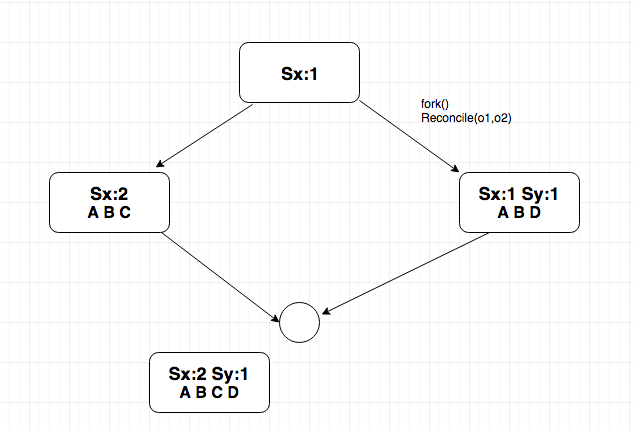
\includegraphics[width=0.5\linewidth]{fig1}
\caption[]{Reconciliation Mechanism}
\label{cpl}
\end{figure}\\
The two main operations offered by Dynamo are: \textit{get(key)} and \textit{put(key, context, value)}. When a client wants to update the value associated with a key, it must specify which version it is updating. This is done by passing the context it obtained from an earlier read operation. On a \textit{get()}, if Dynamo has multiple versions of values for the key and if it cannot automatically resolve them, then it will return all values with its corresponding contexts (versions) to the client. It's up to the client to reconcile the different versions.(fig 1)

For fault tolerance, it follows the concept of Consistent hashing.

\subsection{Anti-entropy}
Anti-entropy refers to the process of coping with decays in a distributed setting. It involves comparing all replicas of each block of data that exist (or is expected to exist) and refreshing each replica if required. The naive way to compare and refresh each replica would involve large data transfer between the replicas which is undesirable. Therefore, we use a data structure named Merkle tree to limit the amount of data transferred when synchronizing. A Merkle tree is a hash tree where leaves are hashes of the values of individual keys. Parent nodes higher in the tree are hashes of their respective children. To compare data in replicas, Dynamo compares their Merkle trees. The comparison starts at the root. If the hashes are the same, the data is already synchronized. Otherwise, the subtrees that is different is compared. This goes on until the leaf node that's not synchronized.(fig 2)

\begin{figure}[h]
\centering
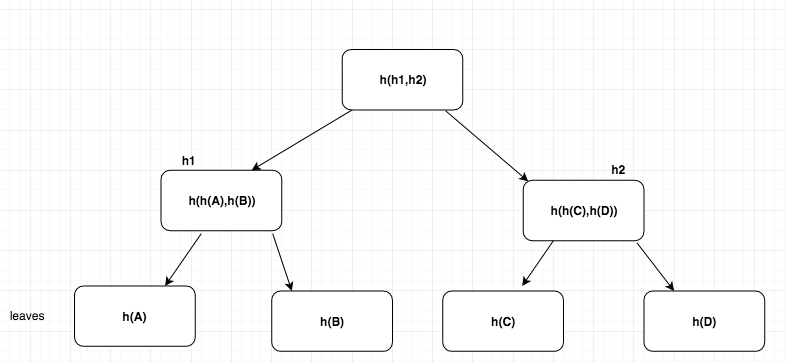
\includegraphics[width=0.5\linewidth]{fig2}
\caption[]{Merkle Tree}
\label{cpl}
\end{figure}\\

\end{document}
